\chapter{Design and Architecture}

The design of software application needs a well defined problem, when a new improved design of a user interface is needed. Main focus lays in easy navigation, responsive interface and intuitive access to the most needed parts of the system. Architecture describes ways of structuring software logic and communication.

\section{Flux and MVC}\label{sec:fluxmvc}
\subsection{What is MVC and Flux}
Two main software design patterns that were considered for this solution were Flux and MVC, React.js was set to be the main tool for using it as a view - (the part of the application that shows current data state), while researching React.js the preferred way to write the app for many programmers seemed to be Flux, although there was no clear advantage of Flux. MVC stands for Model View Controller, the first part, the \emph{model} represents the logic, and data that is being displayed, the \emph{view} is the part that displays the information the current data, and \emph{controller} accepts the user input and sends it either to model or view, these three parts are the main elements of the application that communicate with each other. One can be very creative while implementing MVC, there exists many implementations of MVC, in general the flow inside MVC is not well defined, and when inexperienced programmer tries it, it can become very difficult to manage all the different parts, and it gets especially complicated when having a lot of different components that communicate with each other. Even though Autograder is not as huge and complicated as some of the sites out there, its still not a small application, there are many elements that depend on data from different places. To explain it better let's look at an example. Lab overview where teachers can have an easy access to all the assignments and see individual results.

\begin{figure}[h]
  {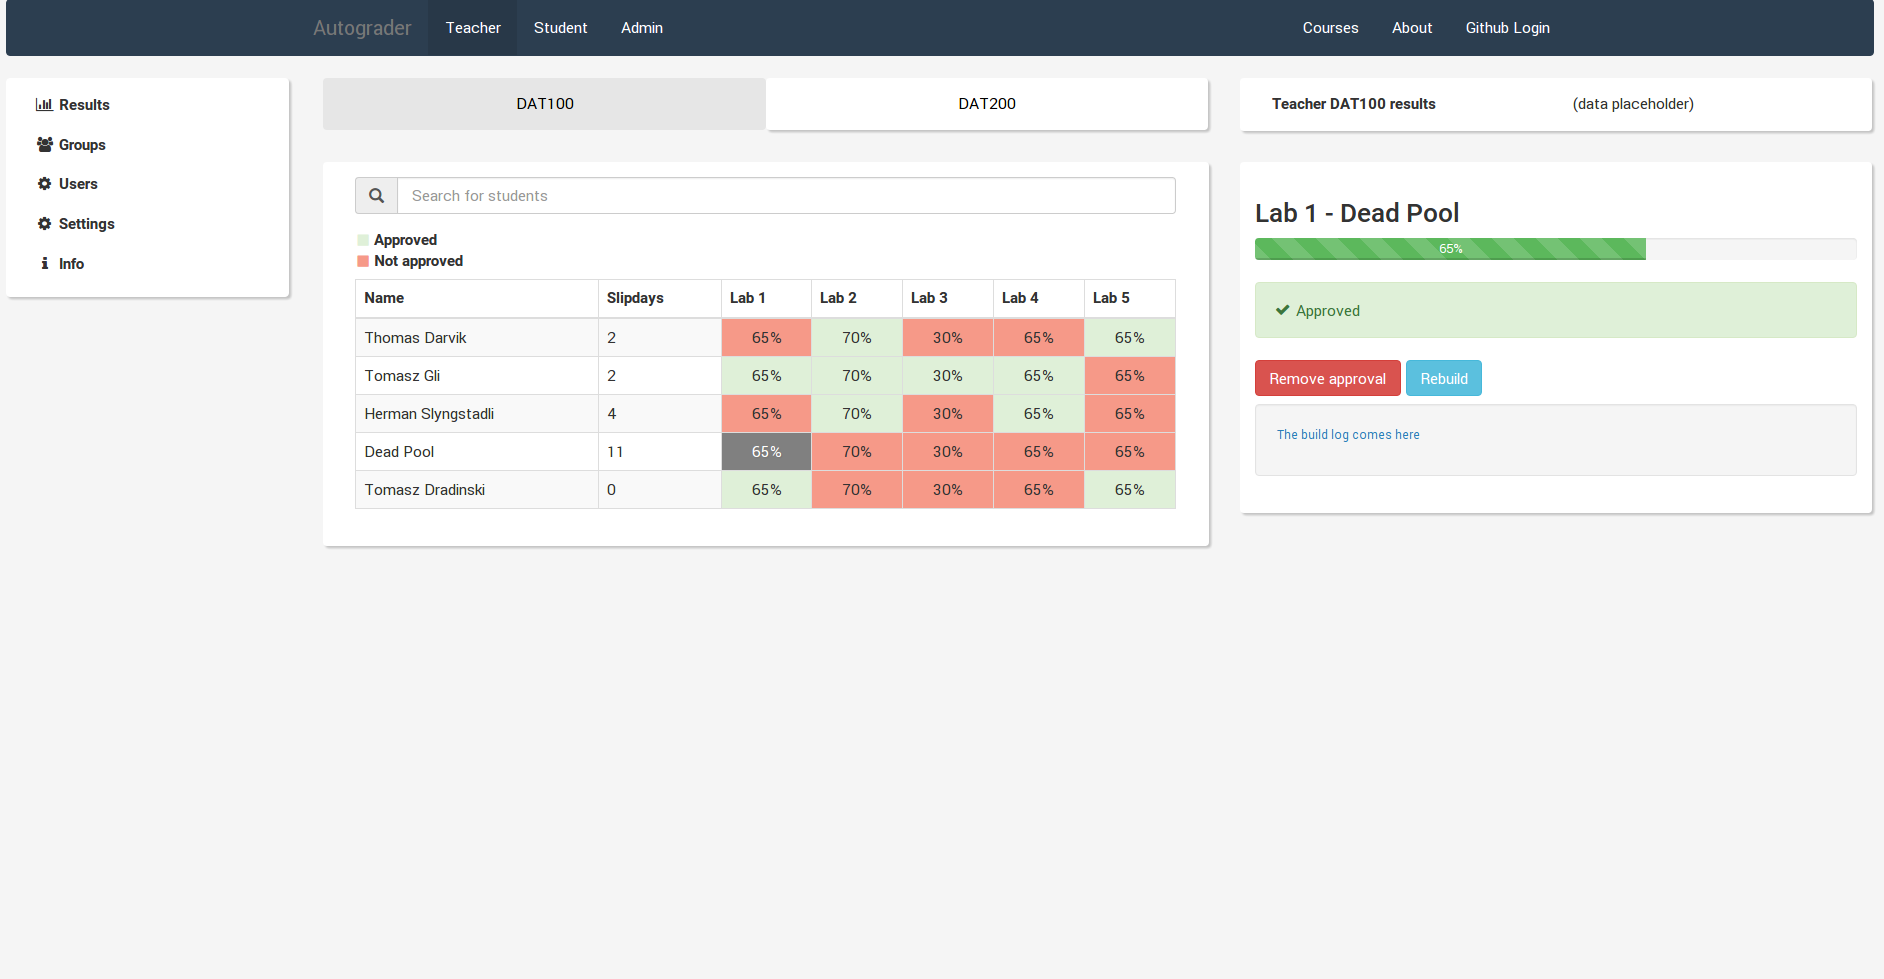
\includegraphics[width=1\linewidth]{laboverviewteacher}}
  \caption{The view that teacher sees when looking at all the labs in a given course}
  \label{fig:laboverwievteacher}
\end{figure}

The center section is a table of all the lab results for every student, to the right there is a expanded view of a selected lab (marked with gray).
Simple flowchart represented with MVC style design:

\begin{figure}[h]
\centering
% Graphic for TeX using PGF
% Title: /home/tomgli/workspace/github.com/bachopp/thesis/files/chapters/design/graphs/modelmvc.dia
% Creator: Dia v0.97.3
% CreationDate: Wed Apr 20 16:35:36 2016
% For: tomgli
% \usepackage{tikz}
% The following commands are not supported in PSTricks at present
% We define them conditionally, so when they are implemented,
% this pgf file will use them.
\ifx\du\undefined
  \newlength{\du}
\fi
\setlength{\du}{15\unitlength}
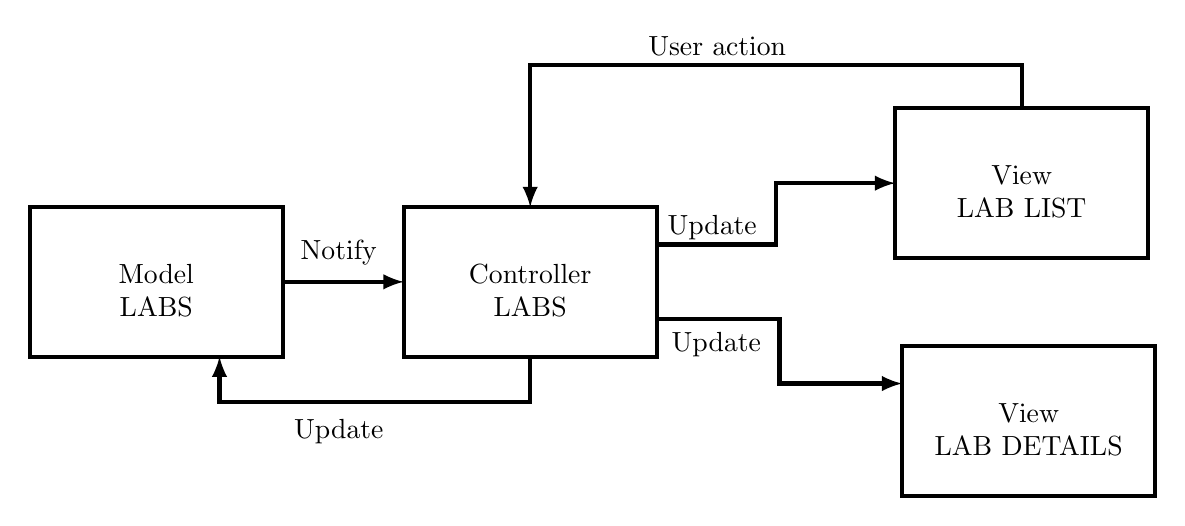
\begin{tikzpicture}
\pgftransformxscale{1.000000}
\pgftransformyscale{-1.000000}
\definecolor{dialinecolor}{rgb}{0.000000, 0.000000, 0.000000}
\pgfsetstrokecolor{dialinecolor}
\definecolor{dialinecolor}{rgb}{1.000000, 1.000000, 1.000000}
\pgfsetfillcolor{dialinecolor}
\definecolor{dialinecolor}{rgb}{1.000000, 1.000000, 1.000000}
\pgfsetfillcolor{dialinecolor}
\fill (29.571900\du,2.356000\du)--(29.571900\du,5.957392\du)--(35.666573\du,5.957392\du)--(35.666573\du,2.356000\du)--cycle;
\pgfsetlinewidth{0.100000\du}
\pgfsetdash{}{0pt}
\pgfsetdash{}{0pt}
\pgfsetmiterjoin
\definecolor{dialinecolor}{rgb}{0.000000, 0.000000, 0.000000}
\pgfsetstrokecolor{dialinecolor}
\draw (29.571900\du,2.356000\du)--(29.571900\du,5.957392\du)--(35.666573\du,5.957392\du)--(35.666573\du,2.356000\du)--cycle;
% setfont left to latex
\definecolor{dialinecolor}{rgb}{0.000000, 0.000000, 0.000000}
\pgfsetstrokecolor{dialinecolor}
\node at (32.619236\du,3.956696\du){View};
% setfont left to latex
\definecolor{dialinecolor}{rgb}{0.000000, 0.000000, 0.000000}
\pgfsetstrokecolor{dialinecolor}
\node at (32.619236\du,4.756696\du){LAB LIST};
\definecolor{dialinecolor}{rgb}{1.000000, 1.000000, 1.000000}
\pgfsetfillcolor{dialinecolor}
\fill (8.724400\du,4.733100\du)--(8.724400\du,8.334492\du)--(14.819073\du,8.334492\du)--(14.819073\du,4.733100\du)--cycle;
\pgfsetlinewidth{0.100000\du}
\pgfsetdash{}{0pt}
\pgfsetdash{}{0pt}
\pgfsetmiterjoin
\definecolor{dialinecolor}{rgb}{0.000000, 0.000000, 0.000000}
\pgfsetstrokecolor{dialinecolor}
\draw (8.724400\du,4.733100\du)--(8.724400\du,8.334492\du)--(14.819073\du,8.334492\du)--(14.819073\du,4.733100\du)--cycle;
% setfont left to latex
\definecolor{dialinecolor}{rgb}{0.000000, 0.000000, 0.000000}
\pgfsetstrokecolor{dialinecolor}
\node at (11.771736\du,6.333796\du){Model};
% setfont left to latex
\definecolor{dialinecolor}{rgb}{0.000000, 0.000000, 0.000000}
\pgfsetstrokecolor{dialinecolor}
\node at (11.771736\du,7.133796\du){LABS};
\definecolor{dialinecolor}{rgb}{1.000000, 1.000000, 1.000000}
\pgfsetfillcolor{dialinecolor}
\fill (17.732600\du,4.733100\du)--(17.732600\du,8.334492\du)--(23.827273\du,8.334492\du)--(23.827273\du,4.733100\du)--cycle;
\pgfsetlinewidth{0.100000\du}
\pgfsetdash{}{0pt}
\pgfsetdash{}{0pt}
\pgfsetmiterjoin
\definecolor{dialinecolor}{rgb}{0.000000, 0.000000, 0.000000}
\pgfsetstrokecolor{dialinecolor}
\draw (17.732600\du,4.733100\du)--(17.732600\du,8.334492\du)--(23.827273\du,8.334492\du)--(23.827273\du,4.733100\du)--cycle;
% setfont left to latex
\definecolor{dialinecolor}{rgb}{0.000000, 0.000000, 0.000000}
\pgfsetstrokecolor{dialinecolor}
\node at (20.779936\du,6.333796\du){Controller};
% setfont left to latex
\definecolor{dialinecolor}{rgb}{0.000000, 0.000000, 0.000000}
\pgfsetstrokecolor{dialinecolor}
\node at (20.779936\du,7.133796\du){LABS};
\definecolor{dialinecolor}{rgb}{1.000000, 1.000000, 1.000000}
\pgfsetfillcolor{dialinecolor}
\fill (29.740800\du,8.083100\du)--(29.740800\du,11.684492\du)--(35.835473\du,11.684492\du)--(35.835473\du,8.083100\du)--cycle;
\pgfsetlinewidth{0.100000\du}
\pgfsetdash{}{0pt}
\pgfsetdash{}{0pt}
\pgfsetmiterjoin
\definecolor{dialinecolor}{rgb}{0.000000, 0.000000, 0.000000}
\pgfsetstrokecolor{dialinecolor}
\draw (29.740800\du,8.083100\du)--(29.740800\du,11.684492\du)--(35.835473\du,11.684492\du)--(35.835473\du,8.083100\du)--cycle;
% setfont left to latex
\definecolor{dialinecolor}{rgb}{0.000000, 0.000000, 0.000000}
\pgfsetstrokecolor{dialinecolor}
\node at (32.788136\du,9.683796\du){View};
% setfont left to latex
\definecolor{dialinecolor}{rgb}{0.000000, 0.000000, 0.000000}
\pgfsetstrokecolor{dialinecolor}
\node at (32.788136\du,10.483796\du){LAB DETAILS};
\pgfsetlinewidth{0.100000\du}
\pgfsetdash{}{0pt}
\pgfsetdash{}{0pt}
\pgfsetbuttcap
{
\definecolor{dialinecolor}{rgb}{0.000000, 0.000000, 0.000000}
\pgfsetfillcolor{dialinecolor}
% was here!!!
\pgfsetarrowsend{latex}
\definecolor{dialinecolor}{rgb}{0.000000, 0.000000, 0.000000}
\pgfsetstrokecolor{dialinecolor}
\draw (14.819073\du,6.533796\du)--(17.732600\du,6.533800\du);
}
\pgfsetlinewidth{0.100000\du}
\pgfsetdash{}{0pt}
\pgfsetdash{}{0pt}
\pgfsetmiterjoin
\pgfsetbuttcap
{
\definecolor{dialinecolor}{rgb}{0.000000, 0.000000, 0.000000}
\pgfsetfillcolor{dialinecolor}
% was here!!!
\pgfsetarrowsend{latex}
{\pgfsetcornersarced{\pgfpoint{0.000000\du}{0.000000\du}}\definecolor{dialinecolor}{rgb}{0.000000, 0.000000, 0.000000}
\pgfsetstrokecolor{dialinecolor}
\draw (23.827273\du,5.633448\du)--(26.699586\du,5.633448\du)--(26.699586\du,4.156696\du)--(29.571900\du,4.156696\du);
}}
\pgfsetlinewidth{0.100000\du}
\pgfsetdash{}{0pt}
\pgfsetdash{}{0pt}
\pgfsetmiterjoin
\pgfsetbuttcap
{
\definecolor{dialinecolor}{rgb}{0.000000, 0.000000, 0.000000}
\pgfsetfillcolor{dialinecolor}
% was here!!!
\pgfsetarrowsend{latex}
{\pgfsetcornersarced{\pgfpoint{0.000000\du}{0.000000\du}}\definecolor{dialinecolor}{rgb}{0.000000, 0.000000, 0.000000}
\pgfsetstrokecolor{dialinecolor}
\draw (23.827273\du,7.434144\du)--(26.784036\du,7.434144\du)--(26.784036\du,8.983448\du)--(29.740800\du,8.983448\du);
}}
\pgfsetlinewidth{0.100000\du}
\pgfsetdash{}{0pt}
\pgfsetdash{}{0pt}
\pgfsetmiterjoin
\pgfsetbuttcap
{
\definecolor{dialinecolor}{rgb}{0.000000, 0.000000, 0.000000}
\pgfsetfillcolor{dialinecolor}
% was here!!!
\pgfsetarrowsend{latex}
{\pgfsetcornersarced{\pgfpoint{0.000000\du}{0.000000\du}}\definecolor{dialinecolor}{rgb}{0.000000, 0.000000, 0.000000}
\pgfsetstrokecolor{dialinecolor}
\draw (32.619236\du,2.356000\du)--(32.619236\du,1.306000\du)--(20.779936\du,1.306000\du)--(20.779936\du,4.733100\du);
}}
\pgfsetlinewidth{0.100000\du}
\pgfsetdash{}{0pt}
\pgfsetdash{}{0pt}
\pgfsetmiterjoin
\pgfsetbuttcap
{
\definecolor{dialinecolor}{rgb}{0.000000, 0.000000, 0.000000}
\pgfsetfillcolor{dialinecolor}
% was here!!!
\pgfsetarrowsend{latex}
{\pgfsetcornersarced{\pgfpoint{0.000000\du}{0.000000\du}}\definecolor{dialinecolor}{rgb}{0.000000, 0.000000, 0.000000}
\pgfsetstrokecolor{dialinecolor}
\draw (20.779936\du,8.384944\du)--(20.779936\du,9.434944\du)--(13.295405\du,9.434944\du)--(13.295405\du,8.334492\du);
}}
% setfont left to latex
\definecolor{dialinecolor}{rgb}{0.000000, 0.000000, 0.000000}
\pgfsetstrokecolor{dialinecolor}
\node at (25.285537\du,0.860839\du){User action};
% setfont left to latex
\definecolor{dialinecolor}{rgb}{0.000000, 0.000000, 0.000000}
\pgfsetstrokecolor{dialinecolor}
\node at (25.163142\du,5.225726\du){Update};
% setfont left to latex
\definecolor{dialinecolor}{rgb}{0.000000, 0.000000, 0.000000}
\pgfsetstrokecolor{dialinecolor}
\node at (25.263132\du,8.056646\du){Update};
% setfont left to latex
\definecolor{dialinecolor}{rgb}{0.000000, 0.000000, 0.000000}
\pgfsetstrokecolor{dialinecolor}
\node at (16.168522\du,5.834114\du){Notify};
% setfont left to latex
\definecolor{dialinecolor}{rgb}{0.000000, 0.000000, 0.000000}
\pgfsetstrokecolor{dialinecolor}
\node at (16.168522\du,10.141612\du){Update};
\end{tikzpicture}

\caption{Example of how the MVC architecture behaves}
\end{figure}

In short, the figure represents only one specific case for implementing certain functionality, there is no general pattern in which data flows through the system, in this case: views signal controller, controller updates model, model notifies about its changes to the controller, then the controller updates the views. This is pretty straight forward, but as the application grows and more components and interactive elements are added it may be difficult to visualize the flow.
\\Flux was design with simplicity in mind, although the pattern may not be as different from MVC at first, key difference is that in Flux the data flow is defined, and every action is forced to the beginning of the system:

\begin{figure}[h]
\centering
\scalebox{0.9}{% Graphic for TeX using PGF
% Title: E:\workspace\go\src\github.com\bachopp\thesis\files\chapters\design\graphs\modelflux.dia
% Creator: Dia v0.97.2
% CreationDate: Sun Apr 24 14:22:10 2016
% For: Tomasz
% \usepackage{tikz}
% The following commands are not supported in PSTricks at present
% We define them conditionally, so when they are implemented,
% this pgf file will use them.
\ifx\du\undefined
  \newlength{\du}
\fi
\setlength{\du}{15\unitlength}
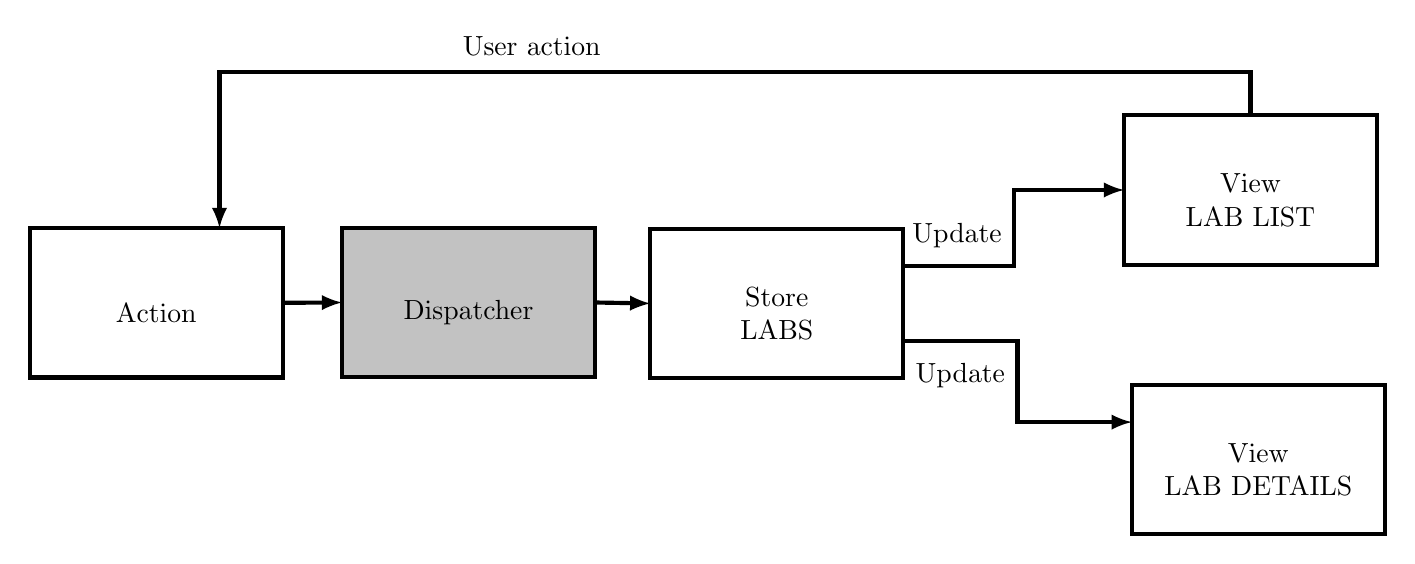
\begin{tikzpicture}
\pgftransformxscale{1.000000}
\pgftransformyscale{-1.000000}
\definecolor{dialinecolor}{rgb}{0.000000, 0.000000, 0.000000}
\pgfsetstrokecolor{dialinecolor}
\definecolor{dialinecolor}{rgb}{1.000000, 1.000000, 1.000000}
\pgfsetfillcolor{dialinecolor}
\definecolor{dialinecolor}{rgb}{1.000000, 1.000000, 1.000000}
\pgfsetfillcolor{dialinecolor}
\fill (30.127000\du,2.450020\du)--(30.127000\du,6.051412\du)--(36.221673\du,6.051412\du)--(36.221673\du,2.450020\du)--cycle;
\pgfsetlinewidth{0.100000\du}
\pgfsetdash{}{0pt}
\pgfsetdash{}{0pt}
\pgfsetmiterjoin
\definecolor{dialinecolor}{rgb}{0.000000, 0.000000, 0.000000}
\pgfsetstrokecolor{dialinecolor}
\draw (30.127000\du,2.450020\du)--(30.127000\du,6.051412\du)--(36.221673\du,6.051412\du)--(36.221673\du,2.450020\du)--cycle;
% setfont left to latex
\definecolor{dialinecolor}{rgb}{0.000000, 0.000000, 0.000000}
\pgfsetstrokecolor{dialinecolor}
\node at (33.174336\du,4.090716\du){View};
% setfont left to latex
\definecolor{dialinecolor}{rgb}{0.000000, 0.000000, 0.000000}
\pgfsetstrokecolor{dialinecolor}
\node at (33.174336\du,4.890716\du){LAB LIST};
\definecolor{dialinecolor}{rgb}{1.000000, 1.000000, 1.000000}
\pgfsetfillcolor{dialinecolor}
\fill (3.767030\du,5.167300\du)--(3.767030\du,8.768692\du)--(9.861703\du,8.768692\du)--(9.861703\du,5.167300\du)--cycle;
\pgfsetlinewidth{0.100000\du}
\pgfsetdash{}{0pt}
\pgfsetdash{}{0pt}
\pgfsetmiterjoin
\definecolor{dialinecolor}{rgb}{0.000000, 0.000000, 0.000000}
\pgfsetstrokecolor{dialinecolor}
\draw (3.767030\du,5.167300\du)--(3.767030\du,8.768692\du)--(9.861703\du,8.768692\du)--(9.861703\du,5.167300\du)--cycle;
% setfont left to latex
\definecolor{dialinecolor}{rgb}{0.000000, 0.000000, 0.000000}
\pgfsetstrokecolor{dialinecolor}
\node at (6.814366\du,7.207996\du){Action};
\definecolor{dialinecolor}{rgb}{0.760784, 0.760784, 0.760784}
\pgfsetfillcolor{dialinecolor}
\fill (11.288700\du,5.160520\du)--(11.288700\du,8.761912\du)--(17.383373\du,8.761912\du)--(17.383373\du,5.160520\du)--cycle;
\pgfsetlinewidth{0.100000\du}
\pgfsetdash{}{0pt}
\pgfsetdash{}{0pt}
\pgfsetmiterjoin
\definecolor{dialinecolor}{rgb}{0.000000, 0.000000, 0.000000}
\pgfsetstrokecolor{dialinecolor}
\draw (11.288700\du,5.160520\du)--(11.288700\du,8.761912\du)--(17.383373\du,8.761912\du)--(17.383373\du,5.160520\du)--cycle;
% setfont left to latex
\definecolor{dialinecolor}{rgb}{0.000000, 0.000000, 0.000000}
\pgfsetstrokecolor{dialinecolor}
\node at (14.336036\du,7.201216\du){Dispatcher};
\definecolor{dialinecolor}{rgb}{1.000000, 1.000000, 1.000000}
\pgfsetfillcolor{dialinecolor}
\fill (18.715500\du,5.183450\du)--(18.715500\du,8.784842\du)--(24.810173\du,8.784842\du)--(24.810173\du,5.183450\du)--cycle;
\pgfsetlinewidth{0.100000\du}
\pgfsetdash{}{0pt}
\pgfsetdash{}{0pt}
\pgfsetmiterjoin
\definecolor{dialinecolor}{rgb}{0.000000, 0.000000, 0.000000}
\pgfsetstrokecolor{dialinecolor}
\draw (18.715500\du,5.183450\du)--(18.715500\du,8.784842\du)--(24.810173\du,8.784842\du)--(24.810173\du,5.183450\du)--cycle;
% setfont left to latex
\definecolor{dialinecolor}{rgb}{0.000000, 0.000000, 0.000000}
\pgfsetstrokecolor{dialinecolor}
\node at (21.762836\du,6.824146\du){Store};
% setfont left to latex
\definecolor{dialinecolor}{rgb}{0.000000, 0.000000, 0.000000}
\pgfsetstrokecolor{dialinecolor}
\node at (21.762836\du,7.624146\du){LABS};
\definecolor{dialinecolor}{rgb}{1.000000, 1.000000, 1.000000}
\pgfsetfillcolor{dialinecolor}
\fill (30.314600\du,8.941950\du)--(30.314600\du,12.543342\du)--(36.409273\du,12.543342\du)--(36.409273\du,8.941950\du)--cycle;
\pgfsetlinewidth{0.100000\du}
\pgfsetdash{}{0pt}
\pgfsetdash{}{0pt}
\pgfsetmiterjoin
\definecolor{dialinecolor}{rgb}{0.000000, 0.000000, 0.000000}
\pgfsetstrokecolor{dialinecolor}
\draw (30.314600\du,8.941950\du)--(30.314600\du,12.543342\du)--(36.409273\du,12.543342\du)--(36.409273\du,8.941950\du)--cycle;
% setfont left to latex
\definecolor{dialinecolor}{rgb}{0.000000, 0.000000, 0.000000}
\pgfsetstrokecolor{dialinecolor}
\node at (33.361936\du,10.582646\du){View};
% setfont left to latex
\definecolor{dialinecolor}{rgb}{0.000000, 0.000000, 0.000000}
\pgfsetstrokecolor{dialinecolor}
\node at (33.361936\du,11.382646\du){LAB DETAILS};
\pgfsetlinewidth{0.100000\du}
\pgfsetdash{}{0pt}
\pgfsetdash{}{0pt}
\pgfsetbuttcap
{
\definecolor{dialinecolor}{rgb}{0.000000, 0.000000, 0.000000}
\pgfsetfillcolor{dialinecolor}
% was here!!!
\pgfsetarrowsend{latex}
\definecolor{dialinecolor}{rgb}{0.000000, 0.000000, 0.000000}
\pgfsetstrokecolor{dialinecolor}
\draw (9.861700\du,6.968000\du)--(11.288700\du,6.961216\du);
}
\pgfsetlinewidth{0.100000\du}
\pgfsetdash{}{0pt}
\pgfsetdash{}{0pt}
\pgfsetbuttcap
{
\definecolor{dialinecolor}{rgb}{0.000000, 0.000000, 0.000000}
\pgfsetfillcolor{dialinecolor}
% was here!!!
\pgfsetarrowsend{latex}
\definecolor{dialinecolor}{rgb}{0.000000, 0.000000, 0.000000}
\pgfsetstrokecolor{dialinecolor}
\draw (17.383373\du,6.961216\du)--(18.715500\du,6.984150\du);
}
\pgfsetlinewidth{0.100000\du}
\pgfsetdash{}{0pt}
\pgfsetdash{}{0pt}
\pgfsetmiterjoin
\pgfsetbuttcap
{
\definecolor{dialinecolor}{rgb}{0.000000, 0.000000, 0.000000}
\pgfsetfillcolor{dialinecolor}
% was here!!!
\pgfsetarrowsend{latex}
{\pgfsetcornersarced{\pgfpoint{0.000000\du}{0.000000\du}}\definecolor{dialinecolor}{rgb}{0.000000, 0.000000, 0.000000}
\pgfsetstrokecolor{dialinecolor}
\draw (24.810173\du,6.083798\du)--(27.468586\du,6.083798\du)--(27.468586\du,4.250716\du)--(30.127000\du,4.250716\du);
}}
\pgfsetlinewidth{0.100000\du}
\pgfsetdash{}{0pt}
\pgfsetdash{}{0pt}
\pgfsetmiterjoin
\pgfsetbuttcap
{
\definecolor{dialinecolor}{rgb}{0.000000, 0.000000, 0.000000}
\pgfsetfillcolor{dialinecolor}
% was here!!!
\pgfsetarrowsend{latex}
{\pgfsetcornersarced{\pgfpoint{0.000000\du}{0.000000\du}}\definecolor{dialinecolor}{rgb}{0.000000, 0.000000, 0.000000}
\pgfsetstrokecolor{dialinecolor}
\draw (24.810173\du,7.884494\du)--(27.562386\du,7.884494\du)--(27.562386\du,9.842298\du)--(30.314600\du,9.842298\du);
}}
\pgfsetlinewidth{0.100000\du}
\pgfsetdash{}{0pt}
\pgfsetdash{}{0pt}
\pgfsetmiterjoin
\pgfsetbuttcap
{
\definecolor{dialinecolor}{rgb}{0.000000, 0.000000, 0.000000}
\pgfsetfillcolor{dialinecolor}
% was here!!!
\pgfsetarrowsend{latex}
{\pgfsetcornersarced{\pgfpoint{0.000000\du}{0.000000\du}}\definecolor{dialinecolor}{rgb}{0.000000, 0.000000, 0.000000}
\pgfsetstrokecolor{dialinecolor}
\draw (33.174336\du,2.450020\du)--(33.174336\du,1.400020\du)--(8.338035\du,1.400020\du)--(8.338035\du,5.167300\du);
}}
% setfont left to latex
\definecolor{dialinecolor}{rgb}{0.000000, 0.000000, 0.000000}
\pgfsetstrokecolor{dialinecolor}
\node at (15.858400\du,0.790717\du){User action};
% setfont left to latex
\definecolor{dialinecolor}{rgb}{0.000000, 0.000000, 0.000000}
\pgfsetstrokecolor{dialinecolor}
\node at (26.105100\du,5.356830\du){Update};
% setfont left to latex
\definecolor{dialinecolor}{rgb}{0.000000, 0.000000, 0.000000}
\pgfsetstrokecolor{dialinecolor}
\node at (26.184500\du,8.726810\du){Update};
\end{tikzpicture}
}
\caption{General data flows in Flux architecture}
\end{figure}

Here a user action is triggered, the dispatcher which is a global central hub of the system, reads what \emph{type} of action is being sent, and notifies the stores about it. Each store represents the data for one or many views, its not a direct mapping of how the data is stored on the server, but it manages itself in a way to represent the data any associated views might need. When an action is triggered and reaches store, store then updates itself with the \emph{change} that was associated with the action, when it is done, it notifies the views about the change. Views when they get notified, they get the data from the stores by accessing it through public store getter methods.
This pattern is very scalable, if we were to add more components, by looking at the graph we only need another box, that sends a User action that will further down the graph modify new or the same store. It becomes easier to manage different components, because everything will at some point go through that central hub called the Dispatcher, this is the starting point of every new \emph{state} that the component is in. The main difference between Flux and MVC is that flux forces unidirectional dataflow, this might seem unnecessary at first, and it is when it comes to small applications, but nevertheless it simplifies the maintenance of the codebase in the long run.

\subsection{Why Flux}
In this application, the use of Flux pattern was a bit experimental, it was suggested by the developers of React.js that Flux works really well with React.js as there are appropriate hooks built in to React that could be used, that works naturally with Flux pattern. \todo{more, or delete it..}

\section{Design}

\subsection{User Interface Design}
The focus of new design lays in improving the user experience. Users of previous system, have shown dislike towards the UI design choices. The new UI is designed is such a way so that both students and teachers have intuitive access to the parts of the system that they use most frequently. There exists student section, teacher section, and also admin section, these major sections are designed so that it is obvious what parts of the system you have access to from the current section you are in. having Autograder in teacher mode, one can easily create a new course and rename it, GitHub integration \ref{gihubintegration} takes care of creating and managing the repositories needed in that course, initial setup of a course is done through a course settings page. The management of students that have joined the course, involves actions like organizing groups, expelling students and approving new students who joined the course, these can be done in the groups page and users page through easily accessible navigation. Most used functionality, by both teachers and teaching assistants is course lab overview. This results page lets a teacher quickly skim through all the students and look if anyone hasn't delivered their assignment yet, or see the score of each assignment, from there, it is also possible to approve or reject any given lab assignment. Another function is to be able to easily control group assignments, and assign students to specific groups. In the groups page, there exists a user friendly interface for creating new groups and adding available students to any given group, users can be notified about which group they have been assigned to, similarly, students can easily create groups that need to be approved by the teachers.
\\Students will utilize Autograder mainly for checking if their assignment has been approved, since handing in of the assignments happens through GitHub integration. The default page for student section is lab overview, in there one can see the current assignment and its progress, it is also worth mentioning that usually one student wont be using Autograder in more than one course, but the system is designed for easy switch between different courses by using tabs to switch current page data with the relevant course information. There is no distinguished mode for teaching assistant, these are often students that are also registered as teachers in different course, this is where Autograder main sections come in handy, while working as a TA, user can switch to teacher mode and has access to the teachers functionality in the courses he teaches, similarly switching to student mode gives quick access to relevant functions in that mode.
\\As for admins of the system, there will usually be a handful of users with admin privileges, admins control access to the major sections of Autograder, when a user registers admins can assign teacher permissions for that user to be able to create new organizations and courses, and of course admins can upgrade other users to admins. Besides that there is a settings panel for admins that enables setting up initial setting for Autograder server, like hostname, passwords etc.

\subsection{Planning of software solutions}
To achieve the goal of better, quicker and more responsive interface, the front-end application is written in JavaScript. By using new emerging open source technologies and libraries like React.js, it enabled quick and easy way to create a responsive user interface. As mentioned in section \ref{sec:fluxmvc} React takes care of the view - what the user sees, and interacts with. What is missing is something to control the user interface and the data structures that it displays. When the view part is out of the way, a couple of decisions has to be made about the rest of the front-end system, in this case, the application is an alteration of so called "one page app", that means user doesn't see the page refresh on any updates, the spin in this implementation is that the user is still provided with the new URL on each state change of the app, this is not usually the case in "on page apps". For this purpose another library was used to help us programmatically change the browsers URL, and associate each state of the app with its own URL. Having access URL might not seem like a big of a deal, but it is very helpful when students or teachers want to link to a specific assignment or course signup page.
\\How the client communicates with the server is not relevant for the chosen Flux architecture and React.js. The communication implemented on this solution is called WebSocket protocol, in short this protocol establishes a constant connection with the server which is used to transfer data both ways in real time, updates can be send to the client from the server, there is no need for client to poll for any data. The connection is established after the initial GET request from the browser, client then asks for an "upgrade" to WebSocket protocol. The way client asks for data, is with a request string that represents the data payload that it is expecting to receive, the server associates every request with piece of data, client can also send additional payload such as username, limit for the size of the data e.g size of array list for pagination. More on WebSocket in section \ref{sec:websocket}.
\subsection{User stories / Wireframes}
User stories are a way to describe what application does, and what it is supposed to do in easy to read short descriptions. The focus here is to give a good foundation of what the applications is being developed for. Since there is a lot of functionality to be implemented, with the help of user stories is is possible to concentrate on one functionality described by that user story at a time. One example of a user story would be \emph{"As a teacher I want to be able to easily create groups for assignments, so that i don't have to approve student created groups."} fig: \ref{fig:groupmanagement}, this describes vaguely what a certain user would like to do with the application, but also can be created as a starting point for improvement to existing solution. It is also possible, by looking at this user story, to create a set of tasks that will guide through the steps of implementation. If there are parts of the system that need to be thought out again, or new solutions are needed to be in place before this functionality can be implemented, it is considered a part of the user story task.
\\Wireframes are a crucial part of user interface design. The point of wireframes is to have something that is easier to change than the code to be developed. Before coming to the programming phase, one can iterate over a lot more design propositions, and is able to change things up easily during this initial or planning phase. Wireframes are foundation of the application being developed, they are not supposed to show the creative design, but rather reflect on the technological and use-related aspects of the application. Before the development of new user story takes action, sketches and drawings of user interface are being produced. This is done to eliminate flaws in the interface design before they are implemented, a couple of iterations of drawing are done and evaluated from the users perspective. When this initial phase is done, more sophisticated drawings or wireframes are being created. These more detailed drawings with descriptions of areas of the interface, describe what certain elements of this user interface do. Serving as a blue print for further developing of the interface.
\newpage
\begin{figure}[h]
  \centering
  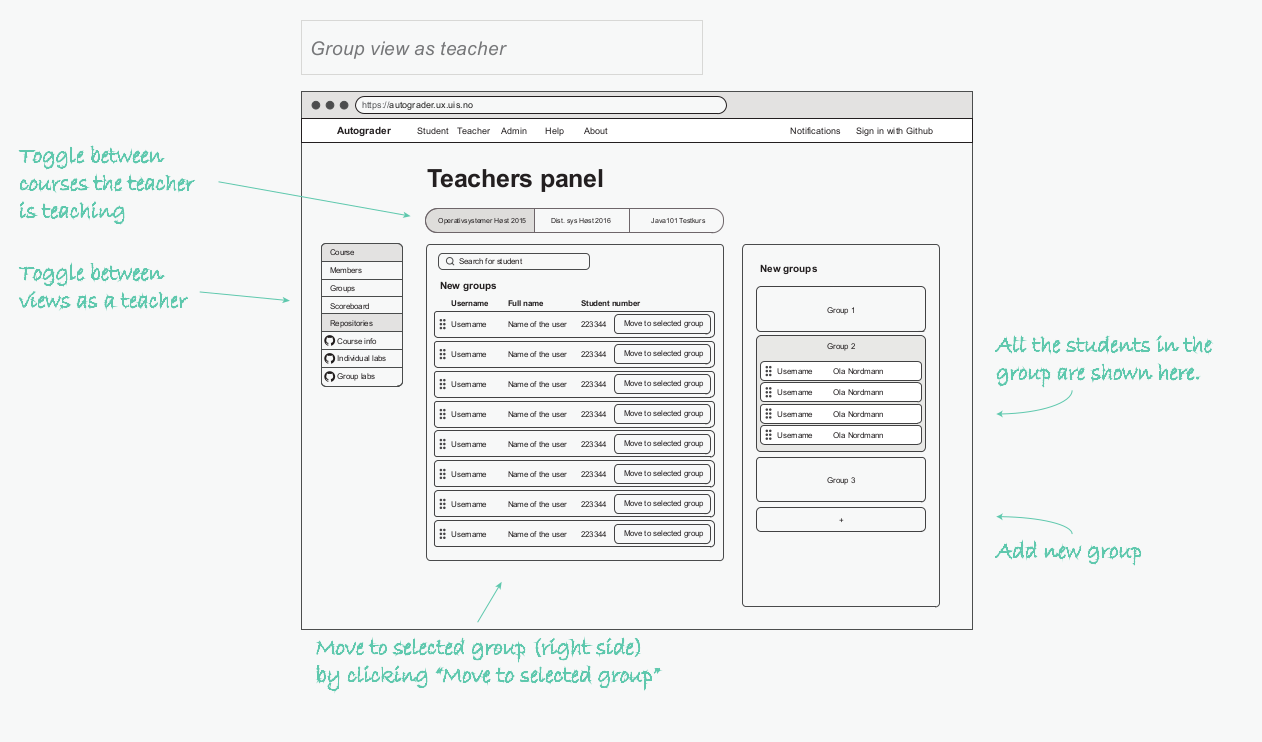
\includegraphics[width=1\linewidth]{groupmanagement}
  \caption{Wireframes for Group management page}
  \label{fig:groupmanagement}
\end{figure}
Wireframes figure above was created as a result of a user story, next step is to create reflection of that Wireframes in code.

\section{Web app}
Architecture of the Autograder system describes the high level structures developed while working on the application. Choice of software architecture, software models on both front and back-end are crucial aspects of creating good application.
\subsection{Software architecture}
Autograder is an application for teachers and students, the new version is going to be running on local university network and is going to be accessible from anywhere on the internet. Primary use for teachers is new creating courses in the system, that are associated with the courses at the university, each course has a GitHub repository associated with it, and configured to the needs of that course. This means that an implementation of GitHub integration needs to be created, this is mainly the focus of back-end part of the software, still the front-end, or web client, needs to be designed in such a way to enable the use of such integration. The client is not supposed to serve as an alternative view of GitHub repositories, GitHub is mainly used as a place to easily store source code, and its login authentication API. The client needs to be able to display courses that a student is enrolled into, assignments that the teacher has published to that course, that also involves group assignments.
\\Although the data is stored in the database, manipulation of that data is done on the client side, and then sent further to the back-end for interpretation and updating the storage. Similarly it is also possible to update the client from the back-end, either directly or through the actions of another client. The user interface updates in real time, as an example, lets take a teacher that is assigning students to group assignments, teacher is using an interactive interface to manipulate the users into selected groups, the student is simultaneously notified in real time when he gets assigned to a new group without the need of refreshing the page, similar things would be new teachers in course, requests for teacher upgrade, deadline and slipdays updates. Teachers can be notified when a new student has enrolled to course, or one of the students has exceeded his slip-days for an assignment. Real time updates are possible due to the connection protocol used in the application. When a client connects to the Autograder server, client application requests for a protocol upgrade, from then on all data transfer is done through \emph{websocket protocol}\cite{websocket}. This enables the server to push its updates to all clients, without being explicitly asked about it by them.
\\The reasoning behind real-time update system was that notifications and responsiveness of user interface was one of the primary reasons for developing this solution. Although one could argue that order methods of updating the UI and notifications would be sufficient, like polling or long-polling - that is frequent client requests for update from the server, websocket protocol has no obvious disadvantages to the presented solution, and at the same time opens possibilities for further upgrades of the system, like chat functionality, which could be utilized for questions related to assignments.
\subsection{Front-end}
Front-end web applications are written in JavaScript, or at least have to be transpiled to JavaScript for the browsers to be able to understand it. Applications in JS, are single threaded...
\todo{single threaded approach}
\subsection{Angular}
\todo{discuss other methods than react, needs more research}
\subsection{React}
\todo{Would we use react for this purpose again?}

\section{Server}
Back-end solution is not the main focus of this application. Nonetheless a working temporary server needed to be put together, as well as database to store mock data and to test the logical functionality of the system on the front-end and the way the data is being communicated between the two ends.
\subsection{Server}
The server is written in Go \emph{Golang}, for this purpose there was no real  preference as to what language to use, but assumptions were made that the final server will also be written in go, therefore it was a clear choice. The Autograder server is going to be handling about 100 clients at once, \worry{not event that many, rewrite later} this is not a big number, but the possibility is that it will grow in the future. The problem that arose during the development was the way in which the server should handle the clients. As discussed earlier, the client requests for protocol upgrade to websocket protocol, this means that only the initial handshake is done through HTTP, this removes any need for further HTTP related requests. Before the websocket were implemented on the client side, the plan was to use a library called gorilla/mux, a multiplexer to easily handle different URL, and assign handle functions to them. When websocket on the client-side where implemented, realization occurred that the multiplexer for HTTP requests will not be used at all, but on the other hand the way to handle the websocket payloads will have to be implemented. \worry{There exists a simple switch statement that handles the payloads through websocket, this will have to be worked on a bit more, as it is now we will not discuss it further at this point in time}
\subsection{Database}
Database is another part not central to the application, but just like the server, it was necessary to implement it so that it becomes easier to see the whole flow of the program.
\\SQL database was designed first in a dia \emph{(drawing program)} \worry{and not changed since}

